\section{Instances de EVE}
\label{parcoursstruct}

\subsection{L'Assemblée Générale}

L'Assemblée Générale possède l'autorité absolue. Elle seule peut prendre des
décisions relevant de grands choix stratégiques. Tout changement statutaire
doit par exemple être soumis à son approbation. Ce fut le cas en 2008 pour le
changement de dénomination demandé par les Universités.

Elle réunit l'ensemble des adhérents,
et les décisions sont prises par vote.
La majorité requise et le quorum fluctuent selon le type de décision.
Pour de très nombreuses raisons,et notamment des quorums trop élevés,
des contraintes matérielles déraisonnables, les statuts ne peuvent être
convenablement appliqués.

Le Bureau arrête l'ordre du jour et assure la tenue des réunions.

Une Assemblée Générale Extraordinaire annuelle approuve les bilans moral et
financier présentés respectivement par le Président et le Trésorier,
et désigne 3 représentants au Conseil d'Administration.

La gestion du fonctionnement au cours de l'année et le traitement de questions
urgentes est délégué au Conseil d'Administration.

\subsection{Le Conseil d'Administration}

Le Conseil d'Administration regroupe :

\begin{itemize}
\item Les Vice-Présidents Étudiants des trois universités grenobloises, de Grenoble INP et du CROUS ;
\item Un représentant par Conseil des Études et de la Vie Universitaire de ces quatre établissements d'enseignement supérieur ;
\item Un représentant de chaque association conventionnée :
	\begin{itemize}
	\item Intègre ;
	\item Radio Campus ;
	\item L'Association Ludique des Étudiants de Grenoble ;
	\item La la Trace Jaune ;
	\item L'Aide Juridique Étudiante ;
	\end{itemize}
\item Cap Berriat ;
\item Trois représentants associatifs élus par l'Assemblée Générale.
\end{itemize}

Sont invités permanents :

\begin{itemize}
\item Grenoble, Université de l'Innovation ;
\item GreCO ;
\item La Métro ;
\item Les présidences des quatre établissements d'enseignement supérieur.
\end{itemize}

Il élit le Bureau en son sein.

\subsection{Le Bureau}

Le Bureau est composé d'un Président, d'un Secrétaire et d'un Trésorier.

\subsection{Le Comité d'Animation}

Le Comité d'Animation regroupe :

\begin{itemize}
\item Les Vice-Présidents Étudiants ;
\item Les représentants associatifs ;
\item Grenoble, Université de l'Innovation ;
\item Le CROUS ;
\item Les représentants des associations conventionnées ;
\item Le responsable du service Pépinière.
\end{itemize}

Il autorise la mise à disposition de locaux et matériel aux associations
et commissions organisant des événements.

\subsection{Commissions}

\subsection{Services}

\subsubsection{ADAM}

ADAM, Aide au Développement des associations Motivées, couramment désignée comme « La Pépinière », dispose de 3 salariés :
\begin{itemize}
\item Un responsable de service, actuellement Véronique Mino ;
\item Un responsable de la communication, qui assure également l'accueil des associations entre 9h et 13h ;
\item Un personnel assurant l'accueil des associations entre 13h et 17h.
\end{itemize}

Elle prend en charge toutes

\subsubsection{Café}

\subsubsection{ENE}

\subsubsection{API}

\subsubsection{Guichet Préfecture}

\section{Diagrammes de gestion}
\subsection{Organigramme}

\subsection{Diagrammes de flux}

\subsubsection{Chaîne de fin de stock au Grand Café}

\begin{center}
\begin{dot2tex}
digraph FinStockBar {
  size = "7";
  rankdir = "LR";
  node [ shape = "circle", style = filled, fillcolor=lightgray ];
  SI [ shape = "octagon" ];
  F [ shape = "doublecircle" ];
  SI -> S [ label = "1" ] ;
  S -> R [ label = "2" ];
  R -> F [ label = "3" ];
  F -> S [ label = "4" ];
  S -> SI [ label = "5" ];
  S -> C [ label = "6" ];
  C -> SI [ label = "7" ];
  C -> F [ label = "8" ];
  C -> SI [ label = "9" ];
}
\end{dot2tex}
\end{center}
\begin{enumerate}
\item Le SI (caisse du Grand Café) indique au S (serveur) une fin de stock ;
\item Le S transmet l'information au responsable stocks (R) ;
\item Le R passe une commande au fournisseur (F) ;
\item F livre le produit, fournit un bon de livraison et une facture au S ;
\item Le S met à jour le stock dans le SI ;
\item Le S transmet le bon de livraison et la facture au comptable (C) ;
\item Le S saisit la facture dans le SI ;
\item Le S effectue le règlement (8) auprès du F ;
\item Le S l'indique au SI.
\end{enumerate}

\subsubsection{Adhésion d'une association à la Pépinière}

Si l'association ne souhaite qu'être référencée sur le site de EVE,
la chaîne s'interrompt à l'étape TODO

\begin{center}
\begin{dot2tex}
digraph AdhesionAsso {
  size = "7";
  rankdir = "LR";
  node [ shape = "circle", style = filled, fillcolor=lightgray ];
  SI [ shape = "octagon" ];
  A [ shape = "doublecircle" ];
  A -> SI [ label = "1" ] ;
  P -> SI [label="2"];
  SI -> A [label="3"];
  A -> P [label="4"];
  P -> SI [label="5"];
  SI -> A [label="6"];
  P -> C [label="7"];
  C -> SI [label="8"];
  SI -> A [label="9"];
}
\end{dot2tex}
\end{center}

%\begin{enumerate}
A info SI
Pep -> si validation
si -> asso mail information
Asso paie -> pep
pep > SI statut adherente
SI  -> asso mail information
Pep -> compta cheque
com -> si (enreg)
si -> asso recu
%\end{enumerate}


\subsection{Exemples de commandes}
\pagebreak
\section{Illustration des outils}
\subsection{Gestion des incidents}
\label{gestion_incidents}
\begin{figure}[!h]
	\centering
	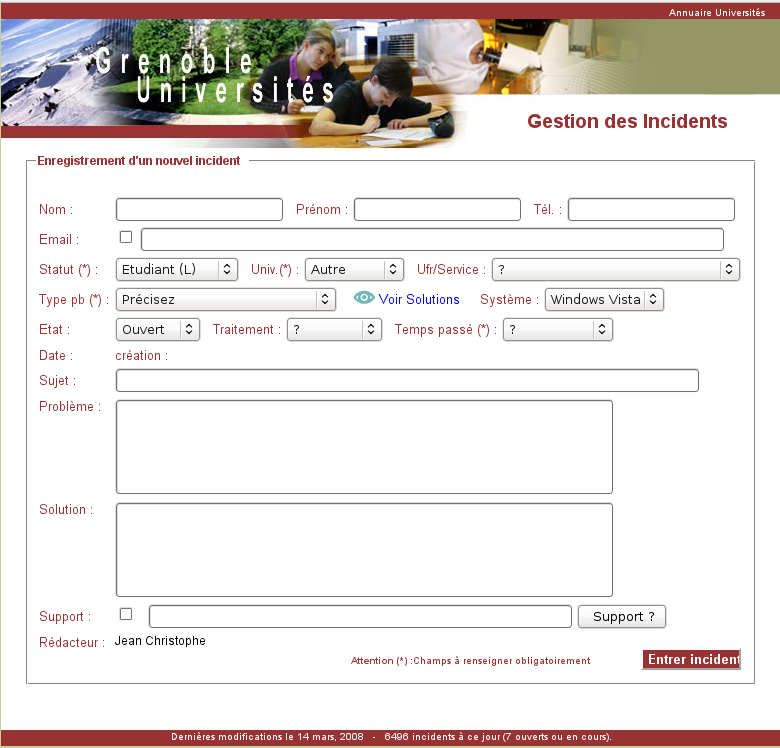
\includegraphics[width=12cm]{annexes/images/gestion_des_incidents.png}
	\caption{Interface de saisie des incidents de l'assistance informatique}
\end{figure}
\clearpage
\section{Modèles et exemples de pièces}
\subsection{A}

